\RequirePackage{luatex85,shellesc}
\documentclass[dvipsnames]{beamer}
\usepackage[subpreambles=false]{standalone}

\usepackage[author={Lyndon White}]{pdfcomment}

\usepackage{fancyvrb}

\usepackage{microtype}
\usepackage{adjustbox}


%\newlength\xunit
%%%%%%%%%%%%%Bibliography
\usepackage[backend=bibtex, url=false,
bibstyle=ieee,firstinits=true]{biblatex}
\renewcommand*{\thefootnote}{} %No symbol or marker
\renewcommand{\footnotesize}{\scriptsize}
%%%%%%%%%%%%%%%%%


\usepackage{xcolor}
\definecolor{chamois}{RGB}{255,255,240}
\definecolor{darkbrown}{RGB}{124,79,0}
\definecolor{UniBlue}{RGB}{83,101,130}

\definecolor{hellgelb}{rgb}{1,1,0.8}
\definecolor{colKeys}{rgb}{0,0,1}
\definecolor{colIdentifier}{rgb}{0,0,0}
\definecolor{colComments}{rgb}{1,0,0}
\definecolor{colString}{rgb}{0,0.5,0}

\usefonttheme{professionalfonts}
\usepackage{tgadventor}
\renewcommand*\familydefault{\sfdefault}
\usepackage[T1]{fontenc}
\usepackage{microtype}


\newcommand{\topline}{%
  \tikz[remember picture,overlay] {%
    \draw[brown,ultra thick] ([yshift=-1.8cm]current page.north west)-- ([yshift=-1.8cm,xshift=\paperwidth]current page.north west);} }

\renewcommand{\topline}{}

\setbeamertemplate{frametitle}{\begin{minipage}[b][1.8cm][c]{\textwidth}%
	\centering%
	\insertframetitle\\\insertframesubtitle
	\end{minipage}}
	

\addtobeamertemplate{frametitle}{}{\topline%
}

\setbeamertemplate{navigation symbols}{}
\setbeamercolor{background canvas}{bg=chamois}
\setbeamercolor{itemize item}{fg=brown}
%\setbeamertemplate{itemize item}{\maltese}
\setbeamercolor{itemize subitem}{fg=brown}
%\setbeamertemplate{itemize subitem}{\begin{rotate}{90}$\diamondsuit$\end{rotate}}

\setbeamercolor{title}{fg=UniBlue}
\setbeamercolor{frametitle}{fg=UniBlue}    
\setbeamerfont{frametitle}{size=\Large}

\setbeamercolor{author}{fg=darkbrown}
\setbeamercolor{institute}{fg=darkbrown}
\setbeamercolor{date}{fg=darkbrown}


\setbeamercolor{structure}{fg=UniBlue}
\setbeamercolor{alerted text}{fg=UniBlue}
\setbeamercolor{alerted text}{fg=UniBlue}
\setbeamercolor{normal text}{fg=darkbrown!50!black}
\setbeamercolor{math text}{fg=darkbrown}
\setbeamercolor{math text displayed}{fg=darkbrown}



\addtobeamertemplate{block begin}{%
	\setlength{\textwidth}{0.8\textwidth}%
}{}
\setbeamercolor{block title}{bg=darkbrown!40,fg=darkbrown!90}
\setbeamercolor{block body}{bg=darkbrown!20,fg=UniBlue}
\setbeamercolor{block title alerted}{bg=yellow!60,fg=red}
\setbeamercolor{block body alerted}{bg=hellgelb!80,fg=UniBlue}

\AtBeginSection[]{
	\begin{frame}
		\vfill
		\centering
		\begin{beamercolorbox}[sep=8pt,center,shadow=true,rounded=true]{title}
			\usebeamerfont{title}\insertsectionhead\par%
		\end{beamercolorbox}
		\vfill
	\end{frame}
}

\setbeamercolor{math text}{fg=bluewrite}
\setbeamercolor{math text displayed}{fg=bluewrite}

\usefonttheme[onlymath]{serif}

\usepackage{amsmath}
\usepackage{mathtools}
\usepackage{amsmath, amssymb, stmaryrd, mathtools}
\DeclareMathOperator*{\argmin}{argmin}
\DeclareMathOperator*{\argmax}{argmax}

\usepackage{xparse,xstring,etoolbox}
% crossref this against notation section
\newcommand{\vv}[1]{\tilde{#1}} % vector
\newcommand{\seq}[1]{\mathcal{#1}} % sequence
\newcommand{\set}[1]{\mathbb{#1}} % set

%%%%%%%%%
% Indexing/sequence indexing
\newcommand{\seqind}[2]{#1^{#2}} % seqence index
\newcommand{\ind}[2]{#1_{#2}} % indexed
\newcommand{\disamb}[2]{#1^{\mathrm{#2}}} %disambiguated

%% Smart indexing and naming
\newcommand{\ifupper}[3]{
    \normalexpandarg
	\exploregroups
	\StrCount{ABCDEFGHIJKLMNOPQRSTUVWXYZ}{#1}[\uppercount]
	\ifnumgreater{\uppercount}{0}{#2}{#3}
}

%smart index
\DeclareDocumentCommand{\ii}{u{_} m}{
	\ifupper{#1}%
	{% just a single uppercase character, i.e. a matrix
		  %make sure the index is the right length
		\StrCount{#2}{,}[\indcount]
		\ifnumgreater{\indcount}{0}
		{ % Got multiple indexes so all good
		 	\ind{#1}{#2}
		}
		{ % Only 1 index so grab the column
		 	\ind{#1}{{:,#2}}
		}
	}%
	{% Not just a single upper case character
		\ind{#1}{#2}
	}
}

\DeclareDocumentCommand{\nn}{u{_} m}{
	\seqind{#1}{#2}
}

\DeclareDocumentCommand{\dd}{u{_} m}{
	\disamb{#1}{#2}
}

% Index of a vector
\DeclareDocumentCommand{\iv}{u{_} m}{\ii{\vv #1}_{#2}}
\DeclareDocumentCommand{\dv}{u{_} m}{\dd{\vv #1}_{#2}}
\DeclareDocumentCommand{\nv}{u{_} m}{\nn{\vv #1}_{#2}}

%exp
\let\oldexp\exp
\renewcommand{\exp}[1]{\oldexp \left( #1 \right)}
\newcommand{\exptwo}[1]{\oldexp_2 \left( #1 \right)}

\newcommand{\softmax}{\mathrm{smax}}

\DeclareMathOperator*{\expectedop}{\mathbb{E}}
\DeclareDocumentCommand{\expected}{u{_} m}{
	\expectedop\limits_{\mathrlap{#2}}
}


\usepackage[at]{easylist}

%%%%%%%%%%%%%%%%%%%%%%%%%%%%%%%%

\bibliography{master.bib}
\let\oldcite=\cite                                                              
\renewcommand{\cite}[1]{\textcolor{bluewrite}{\oldcite{#1}}}

%%%%%%%%%%%%%%%%%%%%%%%%%%%%%%%%
\usepackage{pgfplots}
\usepackage{pgfplotstable}
\usepackage{booktabs}
\pgfplotsset{
	barbase/.style={
		ybar,ymajorgrids, 
		width=0.95\textwidth, height= 5cm,
		bar width=0.6cm,
		axis line style={draw=none},
		x tick style={draw=none},
		ytick = {0.10, 0.15, ..., 0.4},
		ytick pos=left,
	}
}


%%%%%%%%%%%%%%%%%%

\usepackage{tikz}
\usetikzlibrary{positioning}
\usetikzlibrary{chains}
\usetikzlibrary{decorations.pathmorphing}
%\usetikzlibrary{graphs,graphs.standard,graphdrawing,arrows}
%\usegdlibrary{layered, trees, force}

\usepackage{arrayjobx}
\usepackage{xifthen}
\usepackage{textcomp}

\usepackage{graphicx}
\graphicspath{{./figs/}, {./}}
\usepackage[space]{grffile}

\usepackage{trimclip}

%%%%%%%%%%%%%%%%%%%%%%%%%%%%%%%%%%%
% TIKZ stuff

\usepackage{tikz}
\usetikzlibrary{positioning, fit,  shapes.geometric}
\usepackage{ifthen}
\usepackage{etoolbox}

\tikzset{
	backgroundcolor/.style ={fill=white},
	every node/.append style={
		minimum height=7mm,
	},
	labe/.append style={
		%Blue,
		align = center,
		backgroundcolor,
		fill opacity=0.6,
		text opacity=1,
		font={\footnotesize\itshape}	
	},
	layer/.append style={
		draw,
		align = center,
		minimum height=7mm,
	},
	tight/.append style={
		inner sep=0.2mm,
	},
	lookupbox/.append style={
		draw=none,
		append after command={
		       	[shorten <= -0.5\pgflinewidth]
		       	([shift={(-1.5\pgflinewidth,-0.5\pgflinewidth)}]\tikzlastnode.north east)
		       	edge([shift={( 0.5\pgflinewidth,-0.5\pgflinewidth)}]\tikzlastnode.north west) 
		       	([shift={( 0.5\pgflinewidth,-0.5\pgflinewidth)}]\tikzlastnode.north west)
		       	edge([shift={( 0.5\pgflinewidth,-1.5\pgflinewidth)}]\tikzlastnode.south west)            
		       	([shift={( -1.5\pgflinewidth,+0.5\pgflinewidth)}]\tikzlastnode.south east)
		       	edge([shift={(-1.5\pgflinewidth,-0.5\pgflinewidth)}]\tikzlastnode.north east)
		},
		inner sep=0.7mm,
		outer sep=0mm,
		minimum width=25mm
	}
}

\tikzset{%
	->,
	align=center,
	node distance=30mm, sibling distance=25mm, level distance=40mm,
	every edge/.append style = {thick},
	word/.style= {
		bluewrite,
		font=\itshape,
	},
	layer/.style= {
		rectangle, 
		draw
	},
}



%%%%%%%%%%%%%%%%%%%%%%%%%%%%%%%%%%%%%%%%%%%%


% all notes should just be simple item notes.
% I neither need nor want more functionality
\let\oldnote\note
\renewcommand{\note}{\oldnote[item]}

\renewcommand{\emph}{\alert}

%%%%%%%%%%%%%%%%
\newcommand{\countertitle}[1]{\vfill\vfill{\centering \Large \color{bluewrite} #1}\vspace{-0.5cm}}


%%%%%%%%

\newcommand{\mquote}[1]{\textit{``#1''}}

%%%%%

\newcommand{\natlang}[1]{\textcolor{Purple}{\texttt{#1}}}

%%%%%%%%%%%%%%%%%%%%%


\institute{Department of Electical, Electronic and Computer Engineering\\The University of Western Australia}
\date{}
\title{Natural language is \\ unreasonably simple, unreasonably often}
\subtitle{Adding up word embeddings works far too well,\\ why is that?}
\author{
%	\includegraphics[height=2cm]{juliaml}
%	\includegraphics[height=2cm]{juliatext}
%	\includegraphics[height=2cm]{juliastring}
%	\\
%	\vspace{5mm}
	\textbf{Lyndon White}}

\logo{\hfill\includegraphics[scale=0.12]{uwa}\hfill\hspace{0.5cm}}

\begin{document}

\centering %Center everywhere
\frame{\maketitle}
\logo{}

%\begin{frame}{Australia, really it is quiet far away}
%	\note{A considerable distance you might say}
%	\centering
%	\includegraphics[height=0.8\pageheight]{world}
%\end{frame}
%
%\begin{frame}{The University of Western Australia}
%	\includegraphics[width=0.6\textwidth]{uwaphoto}\hfill\null
%	\vspace{-0.1\pageheight}
%	\raggedleft
%%	\null\hfill%
%	\includegraphics[width=0.6\textwidth]{perthphoto}
%\end{frame}

\begin{frame}{We like to think language is very complicated}
	
	\includegraphics[width=\textwidth]{parseegone}
	\vfill
	\includegraphics[width=\textwidth]{parseegtwo}
	\vfill	
	\vfill	
	\countertitle{This is what we do, and complicated models make us feel good and publish well.}
\end{frame}

\begin{frame}{and sometimes language is}
	\vfill
	\natlang{This movie is a truly excellent example of the quality of cinematography this century; for goodness sake, bring back the good old days of real cinema!}
	\vfill
	\natlang{\textcolor{Green}{You shouldn't miss this,\\ that would be the worst mistake.}}
	\vfill
	\natlang{\textcolor{Orange}{It's not that it is was bad,\\ but it wasn't what I hoped for.}}
	
	\countertitle{And so we need the complicated models.}
	\vfill
\end{frame}

\begin{frame}{but sometimes language isn't}
	\begin{itemize}
		\item \natlang{The girl stands on the tennis court.}
		\item Not: \natlang{The tennis court stands on the girl.}
	\end{itemize}
	\vfill
	\pause
	\structure{How do we know?}
	\begin{description}
		\item[World Knowledge:] \natlang{girl} is an \emph{agent}, that can take \emph{actions}% like \natlang{standing}.
		\\
		\hfill OR\hfill\hfill\hfill\null
		\item[Language Modelling:] the trigram \natlang{tennis court stands} never occurs in the Google Books corpus.
	\end{description}
	\countertitle{And so simple methods work}
\end{frame}



\newcommand{\mathtextcolor}{\color{brownwrite}}
\newcommand{\ut}[2]{\underbrace{\text{\mathtextcolor{}{#1}}}_{\mathclap{\text{#2}}}}
\newcommand{\ot}[2]{\overbrace{\text{\mathtextcolor{}{#1}}}^{\mathclap{\text{#2}}}}
\begin{frame}[label=colorscomplex]{and often it looks like it is complicated\\ but isn't}
	\vfill 
	\begin{columns}
		\begin{column}{0.5\textwidth}
			\renewcommand{\mathtextcolor}{\color[rgb]{0.043,0.535,0.529}}
			\begin{equation*}
				\ut{dark}{basic modifier}
				\quad \ot{green}{color modifier}
				\!\!\ut{ish}{meta modifier}
				\quad \ot{blue}{head color}
			\end{equation*}
			
			\vfill
			\renewcommand{\mathtextcolor}{\color[rgb]{0.063,0.651,0.455}}
			
			\begin{equation*}
				\ut{dark}{basic modifier}
				\qquad \; \ot{blu}{color modifier}
				\!\!\ut{ish}{meta modifier}
				\quad \ot{green}{head color}
			\end{equation*}
		\end{column}
	
		\begin{column}{0.5\textwidth}
			\vfill
			\renewcommand{\mathtextcolor}{\color[rgb]{1,0.398,0.314}}
			\begin{equation*}
			\quad \ot{rudd}{\shortstack{color modifier\\ (red)}}
			\!\!\!\ut{y}{meta modifier}
			\quad \ot{coral}{\shortstack{head color\\ (from noun) }}
			\end{equation*}
			\vfill	
		\end{column}
	\end{columns}


	\note{When it comes to color names, you can define a sophisticated grammar, ISCC-NBS defines a fairly basic one. But it isn't really sufficient to capture everything going on with a realistically sized vocabulary}
	
	\note{I'll be back for this example later}
	
	\countertitle{and so using complicated methods leads to worse performance.}
	\vfill
\end{frame}


\begin{frame}{Two (overlapping) types of problems}
	\vfill
	{\Huge 
	Natural Language Generation
	}\\
%	Decoding RNNs\\
	\vfill
	\vfill
	{\color{bluewrite} \Huge
	Natural Language Understanding
	}
%	Encoding RNNs
	\countertitle{We're interested in the latter}
\end{frame}

\begin{frame}{Analogy Algebra is a bit silly}
\begin{columns}
	\begin{column}{0.5\textwidth}
		\resizebox{\textwidth}{!}{\begin{tikzpicture}
			\node(a) {$\i C_{aunt}$};
			\node(b)[above right = of a] {$\i C_{uncle}$};
			\node(c)[below right = of a] {$\i C_{queen}$};
			\node(d)[above right = of c] {$\i C_{king}$};
			
			\draw[->] (b) -- (a) node[labe,midway]{$\i C_{aunt}-\i C_{uncle}$};
			\draw[->] (d) -- (c) node[labe,midway]{$\i C_{queen}-\i C_{king}$};
			\end{tikzpicture}}			
	\end{column}
	\begin{column}{0.5\textwidth}
		\citehere{gladkova2016analogy}\\
		\vspace{1cm}
		\emph{40 subcategories} of knowledge.
	\end{column}
\end{columns}

\countertitle{But: it is a \textbf{sufficient} condition for good separability with consistency}
\end{frame}

\begin{frame}{Word Embeddings capture lexical (word level) semantics}
	\begin{block}{Firth's Criterion: }
		You shall know a word by the company it keep.
	\end{block}
	\vspace{1cm}
	\begin{block}{The Distributional Hypothesis:}
		Words that occur in similar \emph{contexts}, have similar \emph{meanings}.
	\end{block}
\countertitle{You can add them up to represent sentences}
\end{frame}




\begin{frame}{You can just add up word embeddings and uses it as a representation}
	\begin{block}{\normalsize \citehere{acl2018bleuopposedmeaning}}
		\mquote{On classification tasks,  our [LSTM encoder-decoder] models
			are outperformed even by GloVe-BOW, except
			for the NLI tasks\ldots}
	\end{block}
	
	\begin{block}{\normalsize \citehere{ac2018probingsentencevectors}}
		\mquote{Our first striking result is the good overall performance
			of Bag-of-Vectors, confirming early insights
			that aggregated word embeddings capture
			surprising amounts of sentence information\ldots}
	\end{block}
\end{frame}

\begin{frame}{Some reasons why lexical semantics is capturing what looks like sentence semantics.}
	\vspace{-0.5cm}
	\citehere{ac2018probingsentencevectors}\\
	\vspace{0.5cm}
	\begin{itemize}
		\item 	Most words have same \emph{temporal tense} as sentence.
		\item \emph{Nouns and adjectives} both tend to mark \emph{quantities} of same things.
		\item The presence of some words \emph{(Why, Where, etc)} strongly hints at the \emph{structure of the sentence}
	\end{itemize}
	
	\countertitle{Redundant encoding of information in the words}
\end{frame}

\begin{frame}{Content is king}
	\vspace{-0.5cm}
	Considering further \cite{ac2018probingsentencevectors}\\

	\only<1>{\begin{itemize}
			\vspace{0.5cm}
			\item They looked at $3 \times 8  + 5$ models \note{8 different training varients of 3 types of sophisticaed models, plus 5 baselines}
			\item \emph{10 probing tasks} were used to evaluate the models.
			\item Of the \emph{baseline} models SOWE was often the best.
			\item It was rarely better than the best performing \emph{sophisticated model}
			\item \emph{Except} on Word Content \note{Actually, most of the baseline models are better than the fancy models on the word content task, but SOWE beats them on most of tasks.}
		\end{itemize}
	}
	\only<2>{
		When the probing task results are correlated against 12 down stream tasks.\\
		\includegraphics[height=0.6\pageheight]{probing-cor}
	}
	\note{This is not the say that SOWE wins at downstream tasks; I've not seen those results. But it does highlight just how very important capturing surface information is -- lose track of that, and your losing important information.}
	
	\vspace{-0.5cm}
	
	\countertitle{The words people use are the most important part of what they are saying}
\end{frame}

\begin{frame}{SkipGram is the most well known of recent word embedding methods}
	
	\begin{columns}
		\begin{column}{0.5\textwidth}
			\begin{tikzpicture}[]
			
			
			\coordinate(w1) at (0,0);
			\node[draw,circle,green,left=0.8 of w1](ww1) at (0,0) {$\n w_{i}$};
			
			
			\coordinate[above left=of w1, xshift=-0.95cm, yshift=-1cm] (CC0);% at (Cn);
			\embtable{C}{CC0}{\tiny Input Embs}
			
			\draw[->] (ww1) -- ({C}3.east);
			
			
			\node(L2)[layer, above = 3 of w1,
			%	label={[label distance=0] 0: i.e. \\ $\i \softmax(\ldots)_{\n w_j}$}
			]{
				$\frac{\exp{\i V_{\n w_j, :} \i C_{\n w_i}}}%
				{\sum_{\forall v \in \set V} \exp{\i V_{v, :} \i C_{\n w_i}}}$
			};
			
			\draw[->]  ({C}3.east) -- node[labe]{$\i C_{\n w_i}$} (L2);
			
			
			\node(out)[above = 1.5 of L2]{$P^\star(\n w_j \mid \n w_i)$};
			\draw[->] (L2) edge (out);
			
			
			\coordinate[above = 3 of {C}n] (VV0);
			\embtable[T]{V}{VV0}{\tiny Output Embs}
			
			
			%	\pgfmathsetmacro\ang{(\ii * -2 + -180+20 };
			%	\draw[->] (V\ii.east) -- (L2.\ang);
			%\draw[->] ({V}n.east) -- (L2.south west);
			
			
			%\draw[->] (out.204) -- ({V}6.east);
			\node(ww2)[draw,circle, green, left=0.2 of out]{$\n w_j$};
			\draw[->] (ww2) -- ({V}6.east);
			\draw[->] ({V}6.east)-- node[auto, labe]{$\i V_{\n w_j,:}$} (L2.170);
			\end{tikzpicture}
		\end{column}
		
		\begin{column}{0.5\textwidth}
			\only<1>{
				\begin{align*}
				P^\star&(\n w_j \mid \n w_i) = \i {\softmax \left( V\,\i C_{\n w_i}) \right)}_{\n w_j} \label{equ:skipgram}\\
				&=\frac{\exp{\i V_{\n w_j, :} \i C_{\n w_i}}}%
				{\sum_{\forall k \in \set V} \exp{\i V_{k, :} \i C_{\n w_i}}}
				\end{align*}\\
				\vspace{1cm}
				Maximise $P^\star(\n w_j \mid \n w_i)$
				for combinations of words\\ $\n w_j$, $\n w_i$
				that actually co-occur.\\
				\vspace{1cm}
			}
			\only<2>{
				$P^\star(\n w_j \mid \n w_i)$ is maximised
				when $\i V_{\n w_j, :} \i C_{\n w_i}$
				is maximized.\\
				\vspace{1.7cm}
				i.e. when the \emph{dot-product} of the \emph{input embeddings} and the \emph{output embeddings} of collocated words\\ approaches $1$
			}
		\end{column}
	\end{columns}
	
\end{frame}

\newcommand{\monoto}{\varpropto}%{\raisebox{-0.2em}{\overset{\approx}{\propto}}}
\begin{frame}{SkipGram is a iterative algorithm for weighted collocation matrix factorization.}
	\begin{columns}
		\begin{column}{0.55\textwidth}
			$V$ is a $300\times |\set V|$ {\small input emb matrix}\\
			$C$ is a $|\set V|\times 300$ {\small output emb matrix}\\
			$X$ is a $|\set V|\times |\set V|$ {\small collocation  matrix}\\
			$f$ is some monotonic function.\\
			(\cite{levy2015lsaisbasicallyskipgramswithexperimentstoprove})
		\end{column}
		\begin{column}{0.4\textwidth}
			\begin{align*}
			Loss & \monoto \Vert  X \odot \exp{- V C} \Vert\\
			& \monoto{} \Vert \log (X \odot \exp{- V C}) \Vert\\
			& \monoto{} \Vert \log X - VC \Vert\\
			& \monoto{} \Vert f(X) - VC \Vert
			\end{align*}
			Loss is minimized when  $VC \approx f(X)$
		\end{column}
	\end{columns}
	
	
	\note{Chasing down exactly what that weighting function $f$ is is a bit hairy, as there are many implementation factors like negative sampling, subsampling, etc that go into it. Levy et al, and several others have done it, and it comes out as a proxy for mutual information}
	
	\note{Oh look is is GloVE}
	
	\countertitle{When trying to factorize very large matrices numerical linear algebraticians often use iterative methods.}
	\vfill
\end{frame}



\begin{frame}{So SkipGrams are a \\ dimensionality reduction algorithm,\\ that tries remember collocated words}
	\begin{itemize}
		\item Contrast: \emph{PCA} is a dimensionality reduction algorithm, that tries to \emph{remember the most variant factors}
		\item Contrast: \emph{t-SNE} is a dimensionality reduction algorithm, that tries to \emph{preserve similarity as distance}
		\item Compressing knowledge of collocated words into a dense vector, gives us \emph{Firth's Criterion}.
	\end{itemize}
	
\end{frame}


\begin{frame}{Sums of embeddings actually link to intersection of collocation probabilities}
$w$ and $u$ being words\\
$C$ being an embedding matrix\\
$\set V$ being the vocabulary\\
\begin{align*}\
\i C_w &\propto \log P(\set V \mid w)\\
\i C_u &\propto \log P(\set V \mid u)\\[0.5cm]
%
\therefore \i C_w + \i C_u &\propto \log P(\set V \mid w) + \log P(\set V \mid u) \\
&= \log P(\set V \mid w) \cdot P(\set V \mid u)\\
&\propto  \log P(\set V \mid w \cap u)
\end{align*}

\citehere{mikolovSkip}
\end{frame}


\begin{frame}{Matrix product with onehot vector is\\ indexed slicing}
	Consider the \emph{onehot} representation of some word $w$,\\
	as $\iv e_w=\big[0, \ldots, \underbrace{1}_{\mathclap{w\text{th position}}},0 \ldots, 0\big]$\\
	\vspace{0.5cm}
	It's word embedding is given by
	$\i C_{w} = C^\intercal e_w$
\end{frame}



\begin{frame}{Sum of word embeddings is the same as \\ matrix product with bag of words}
	A bag of words can be represented as a vector of the counts of each word in the vocabulary.\\ \vspace{0.5cm}
	For a sequence of words: $\left(\n w_1, \n w_2, \ldots \right)$ \\\vspace{0.5cm}
	The\emph{ bag of words} can be given by\\ $\v x = \sum_{\forall i} \iv e_{\n w_i}$.\\\vspace{0.5cm}
	
	The \emph{sum of word embeddings} for the same sequence is:
	$\sum_{\forall i} \i C_{\n w_i} = C^\intercal \sum_{\forall i} \iv e_{\n w_i}$
\end{frame}

\begin{frame}{Concatenation followed by matrix product\\ is the same as \\matrix product followed by addition}
	\vspace{-0.7cm}
	\begin{equation*}
	\left[\begin{array}{cc}
	U & V\end{array}\right]\left[\begin{array}{c}
	\v a\\
	\v b
	\end{array}\right] = U\v a + V \v b
	\end{equation*}
	Thus
	\begin{align*}
	C (\v a + \v b) &= 
	C\v a + C \v b \\&=
	\left[\begin{array}{cc}
	C & C\end{array}\right]\left[\begin{array}{c}
	\v a\\
	\v b
	\end{array}\right]
	\end{align*}
	\countertitle{A summed input is the same as a concatenated input\\ with blockwise weight tying.}
	\vfill
	\vfill
	\vfill
	\vfill
	\vfill
\end{frame}

\begin{frame}{We are now going to take a very short break}
	\centering
	\includegraphics[width=\textwidth]{break}	
\end{frame}


\pgfplotstableread[col sep=comma,header=has colnames]{data/selection_len_scores.csv}{\sellenscores}
\begin{frame}[fragile]{Bag of words information is not lost in sums of word embeddings}
	\only<1>{
		\begin{itemize}
			\item A bag of words captures all unigram information in a sentence/document etc
			\item A greedy method can (mostly) recover the BOW from a SOWE\\
			\citehere{White2015BOWgen}
			\begin{enumerate}
				\item Greedily add nearest word to remaining the SOWE to bag
				\item Check each word in bag and swap it for a better one
				\item Repeat until no change.
			\end{enumerate}
			\normalsize
			\item Thus, SOWE captures similar \emph{most} unigram information.
			%\item little cancellation or obscuring sums.
			\note{Further, the SOWE space is (in some sense) \emph{nice}}
		\end{itemize}
	}
	\only<2>{
		\begin{tikzpicture}
		\begin{axis}[xlabel=Ground Truth Sentence Length,
		ylabel=Mean Jaccard Index,
		legend style={at={(0.5,1)}, anchor=south,legend columns=3, draw=none},
		width=10cm,height=4cm,cycle list name=exotic]
		\addplot table [y=brown_glove50_jaccard_mean,x=ground_len]{\sellenscores};
		\addplot table [y=brown_glove100_jaccard_mean,x=ground_len]{\sellenscores};
		\addplot table [y=brown_glove200_jaccard_mean,x=ground_len]{\sellenscores};
		\addplot table [y=brown_glove300_jaccard_mean,x=ground_len]{\sellenscores};%
		\addplot table [y=books_0_01_glove300_jaccard_mean,x=ground_len]{\sellenscores};
		\legend{\small 50D Brown, \small 100D Brown, \small 200D Brown, \small 300D Brown, \small 300D Books}					
		\end{axis}
		\end{tikzpicture}
	}
	\vspace{-0.5cm}
	
	\countertitle{We can reliably recover all words from a sum of word embeddings}
\end{frame}

\begin{frame}{Sentence embeddings space should partition readily according to paraphrases}
	\begin{itemize}
		\item \emph{Paraphrases} are defined by \emph{bidirectional entailment}.
		\item This is an \emph{equivalence relation}
		\item It thus gives rise to a \emph{partition} of \emph{natural language space}.
	\end{itemize}
	\countertitle{}
\end{frame}

\begin{frame}{What does it mean to partition readily?}
	There are many ways one could define the quality of a space, on its ability to be partitioned according to anther linked space's partitions.\\
	%	Without restrictions an arbitrary bijection could be allowed.\\
	%	But that would not be a 
	\note{This is a bit like assessing quality of clusters. And there is prove-ably no ideal cluster qualuty measure}
	
	\begin{description}%[labelsep=1em]
		\item[Convex]\qquad No twists, bulges, holes, jumps etc.
		\item[Seperable]\qquad Should not overlap, should be separate      			
		\item[Concentrated]\quad small area		
	\end{description}
	\countertitle{Notice: these are the same criteria needed linear SVM to work well.}
\end{frame}

\pgfplotstableread[col sep=comma]{
	Name,MSRP,Opiniosis, void
	PV--DM, 78, 38.26,0
	PV--DBOW, 89.93, 32.19,0
	URAE, 51.14, 20.87,0
	%	MOWE, 97.91, 69.30,0
	SOWE, 98.02, 68.75,0
	BOW, 98.37, 65.23,0
	PCA--BOW, 97.96, 54.43,0
}\resultstable

\begin{frame}[fragile]{When assessing ability to match partitions using a linear SVM classification task}
	\begin{tikzpicture}
	\begin{axis}[barbase,
	nodes near coords, nodes near coords align={vertical},
	nodes near coords={\small \hspace{1mm} \pgfmathprintnumber[precision=0]{\pgfplotspointmeta}\%},
	ytick= {0,25,50,75,100},
	yticklabels={0\%,25\%,50\%,75\%,100\%},%\pgfmathprintnumber{\tick}\,\%,
	ybar=1pt,% interval= 0.7,
	ylabel=Accuracy,
	ymin=0, ymax=115,
	%    		enlarge y limits=0.2,
	enlarge x limits=0.1,
	xtick=data,
	xticklabels={PV\\DM,PV\\DBOW,URAE,SOWE,BOW,PCA\\BOW},
	xticklabel pos=lower,
	xticklabel style={align=center},
	legend style={at={(0.5,-0.4)}, anchor=north,legend columns=2, draw=none},
	legend image code/.code={%
		\draw[#1] (0cm,-0.2cm) rectangle (0.5cm,0.3cm);
	}
	]
	\addplot[style={top color=Red, bottom color=Orange, draw=none, mark=none}] table [y=MSRP,x expr=\coordindex, meta=Name] {\resultstable};
	\addplot [style={top color=Blue, bottom color=Cyan, draw=none, mark=none}] table [y=Opiniosis,x expr=\coordindex]{\resultstable};
	\legend{MSRP\hspace{1cm}, Opinosis};
	\end{axis}
	\end{tikzpicture}
	\vspace{-0.7cm}
	\countertitle{Knowing word content is really useful}
\end{frame}



\begin{frame}{What is going on here?}
	\begin{block}{PV-DM / PV-DBOW \\ \citehere{le2014distributed}}
		\mquote{It shows that the paragraph vectors, when evaluated correctly, do not work better than bag-of-words (bag-of-ngrams being even better)}\\
		\hfill -- Tomas Mikolov (23/11/17) w.r.t \cite{mesnil2014ensemble}
	\end{block}
	
	\begin{block}{URAE\\
			\citehere{SocherEtAl2011:PoolRAE}
		}
		Only 200D so not entirely fair.\\
		Based on binary constituency parse structure\\
		Deep, compressing each layer, 2 inputs to one output.
	\end{block}
\end{frame}

\begin{frame}{What is going on here?}
	\begin{block}{BOW \\ Bag of Words}
		Several thousand dimensions\\
		1000D spaces tend to be very separable\\
		No synonym capacity\\
	\end{block}
	\begin{block}{PCA BOW \\ Principle Component Analysis \cite{hotelling1933analysis}}
		Drop down to 300D to match others\\
		PCA is inferior to GloVE as a dimensionality reduction technique,
		for semantic preservation.
	\end{block}
\end{frame}


\begin{frame}[fragile]{Consider machine captioning evaluation}
	Correlation with human ranking in the COMPOSITE captioning evaluation dataset. \cite{Aditya2017COMPOSITE}
	
	\begin{itemize}
		\item For each image, there are 5 captions.
		\item A mix of \emph{human} generated
		\item  and \emph{machine} generated.
		\item this is an evaluation of \emph{evaluation metrics}
		
	\end{itemize}
	\note{To steal someone else's joke. This is a second order evaluation. A first order evaluation is the application of a metric; a third order evaluation is what you are doing now.}
	\countertitle{Task is to rate the captions in the same order as the human rankers.}
\end{frame}


\begin{frame}[fragile, label=captioningres]{Look what wins}
	\vspace{-0.5cm}
	\pgfplotstableread[header=has colnames,
	columns/Method/.style={string type},
	columns/Type/.style={string type}
	]{%
		Method	Kendall	Type
		BLEU	0.191	{basic ngram}
		ROGUE-L	0.213	{basic ngram}
		\emph{GloVE}	0.337	{MOWE}
		METEOR	0.341	{fancy ngram}
		CIDEr	0.342	{fancy ngram}
		SPICE	0.349	{semantic parsing}
		\emph{Word2Vec}	0.349	{MOWE}
		%SPICE+CIDEr	0.357	{semantic parsing}
		\emph{FastText}	0.364	{MOWE}
	}{\compositeCaptionEval}
	
	
	
	\begin{tikzpicture}
	\begin{axis}[barbase,
	xticklabels from table={\compositeCaptionEval}{Method},
	legend style={at={(0.5,-0.7)}, anchor=north,legend columns=2, draw=none},
	legend image post style={xscale=1, yscale=1},
	%	enlargelimits=0.3,
	ylabel = {Kendall's $\tau$\\},
	ymin=0.0, ymax=0.4,
	enlarge x limits=0.1,
	xticklabel style={rotate=90},
	xtick = data,
	%yticklabel={$\mathsf{\pgfmathprintnumber{\tick}}$\small\%},
	nodes near coords={\small \color{brownwrite} $\mathsf{\pgfmathprintnumber[precision=3]{\pgfplotspointmeta}}$},
	]
	
	\addplot[style={top color=Orange, bottom color=Blue, draw=none, mark=none}] table[x expr=\coordindex, y=Kendall]{\compositeCaptionEval};
	
	\end{axis}
	\end{tikzpicture}
	
	{\small
		\textasteriskcentered Forthcoming publication \emph{Naeha Sharif, Lyndon White, Mohammed Bennamoun, Wei Liu, and Syed Afaq Ali Shah}.
	}
	\vspace{-0.1cm}
%	
%	\note{This is a hard task, somewhere between abstractive summarization and machine translation, and the assessment is also difficult.}
%	\note{The similarity to abstractive summarization makes it particular bad -- it is not clear what should be said}
%	\note{Shown here is a comparason of minimum cosine similarity to reference MOWE for different embeddings with more traditional metrics}
%	\note{See that the performance of the traditional ngram based metrics BLEU for MT and ROGUE for summarization kinda suck}
%	\note{Next best is the worst performing out of word embedding models GloVE.}
%	\note{It gets out performed by METEOR and CIDEr, which I would summarize as fancy ngram methods, with synonyms and weights.}
%	\note{Then comes SPICE. SPICE is very sophisticated, it does parsing and builds this semantic graph, then does graph comparasons.}
%	\note{But it is beated by Word2Vec, and by FastText}
%	\note{There are a few reasons why FastText is better than word2vec -- it could be the capturing of morphemes for example. But I'd probably attribute it to a few more years of engineering and a whole lot more data.}
%	
	\countertitle{Captioning quality can be assessed on \textbf{fluency} and on \textbf{adequacy}}
\end{frame}



\begin{frame}{All captions in COMPOSITE are \textbf{fluent}}
	\begin{itemize}
		\item We are really good at language modelling now.
		\item In theory our RNN language models can capture all needed state
		\item COMPOSITE captions are a mix of \emph{human generated} and \emph{state-of-the-art machine generated}.
	\end{itemize}
	\vfill
	\countertitle{Trying to capture fluency in your captioning metric is thus not important}
\end{frame}


\begin{frame}{The proper way to look at adequacy is to build a semantic graph, and apply reasoning to it}
	% TODO replace this with nice figures I made myself
	\begin{columns}
		\begin{column}{0.5\textwidth}
			\includegraphics[width=\textwidth]{spicegraph}
		\end{column}
		\begin{column}{0.5\textwidth}
			This is what SPICE does \note{The best performing model other than a MOWE}.
			(\cite{spice2016})\\
			\vspace{0.5cm}
			You could use AMR (\cite{Banarescu13abstractmeaning}), or ERS (\cite{bender2015ERS}).\\
			
			To get to a form that reasoning can be applied on.
			\note{Or more generally that a neural network can leverage.}
		\end{column}
	\end{columns}
	
	\countertitle{This semantic graph must be derived from the \textbf{right words} in the \textbf{right order}}
\end{frame}


\begin{frame}{The proper way to assess adequacy is a semantic graph}
	\begin{itemize}
		\item The syntactic graph comes from the \emph{word order} and \emph{word content}.
		\item In theory, \emph{different} words in \emph{different} orders could give the \emph{same} semantic graph
		\item and the \emph{same} words in a \emph{different} order could give a \emph{different} semantic graph.
	\end{itemize}
	\countertitle{Semantic graph comes from syntactic graph}
\end{frame}

\begin{frame}{Due to ambiguity in possible word order semantic meaning should not be derivable from averaged lexical meaning representation}
	\begin{itemize}
		\item Well written sentences are short: \emph{14-17 words}
		\item They don't have complicated clauses and negations.
		\item Words are used in consistent phrases:
		\begin{itemize}
			\item \natlang{The girl stands on the tennis court}
			\item Not: \natlang{The tennis court stands on the girl}
		\end{itemize}
		\item Good captions are such good sentences.
		
	\end{itemize}
	\countertitle{But in-practice, it probably is}
\end{frame}

\begin{frame}{Word order is more predictable than you may think}
	\begin{itemize}
		\item Consider some sentence; can you rearrange the \\
		\emph{words} and \emph{punctuation} and make \emph{new sentence}
		\item Is it \emph{grammatical}?
		\item Is it a \emph{paraphrase}?
		\item Is it \emph{likely} (or \emph{sensible}) based on world knowledge?
		\item Was it following some standard transform, like just swapping to proper nouns?
	\end{itemize}
\end{frame}

\begin{frame}{You can recover most probable sentence order from bag of words}
	\citehere{White2016a}
	\begin{itemize}
		\item Using a \emph{language model} you can evaluate the probability of any given order for a bag of words.
		\item With an appropriate \emph{optimization/search} technique you can find the most likely order
		\item This particular work was a simple \emph{trigram language model}
		\note{If this works then a better language model can do better}
	\end{itemize}
	\countertitle{Not a great way to generate sentences, though}
\end{frame}

\begin{frame}{For trigram language models, word ordering is a variation of travelling salesman}
	\resizebox{0.95\textwidth}{!}{\documentclass{standalone}
\usepackage{arrayjobx}
\usepackage{xifthen}
\usepackage{tikz,textcomp}
\usepackage{ amssymb }

\begin{document}
	
\tikzset{ shorten <>/.style={ shorten >=0.2cm, shorten <=0.2cm } }

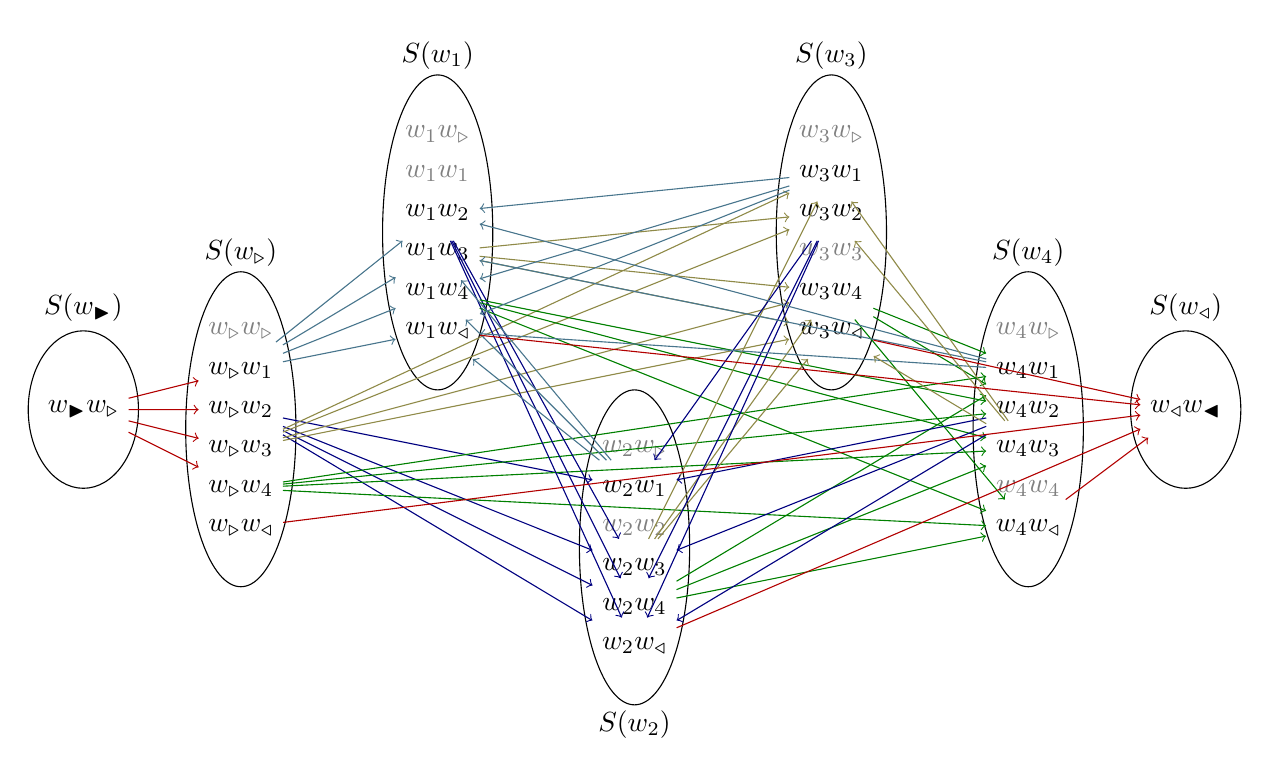
\begin{tikzpicture}
\newarray\Words
\readarray{Words}{$w_\triangleright$&$w_1$&$w_2$&$w_3$&$w_4$&$w_\triangleleft$}
\dataheight=5

\newcommand{\ystep}{0.5}

\newcommand{\gx}{}
\newcommand{\gy}{}


\newcommand{\drawgroupinner}{
	\foreach \j in {1,...,6}
	{
		\colorlet{MyColor}{black}%
		\ifthenelse{\i=\j}{\colorlet{MyColor}{gray}}{}
		\ifthenelse{\j=1}{\colorlet{MyColor}{gray}}{}
		
		\node[MyColor] (w_\i\j) at (\gx,\gy-\ystep*\j cm) {\Words(\i)\Words(\j)};
	}
	\draw (\gx,\gy-3.5*\ystep cm) ellipse (0.7cm and \ystep*4 cm);
}

\newcommand{\drawgrouptop}[3]{%
	\renewcommand{\i}{#1}
	\renewcommand{\gx}{#2 cm}
	\renewcommand{\gy}{#3 cm}
	\drawgroupinner{}	
	\node at (\gx,\gy+1*\ystep cm) {$S($\Words(\i)$)$};

}
\newcommand{\drawgroupbottom}[3]{%
	\renewcommand{\i}{#1}
	\renewcommand{\gx}{#2 cm}
	\renewcommand{\gy}{#3 cm}
	\drawgroupinner{}	
	\node at (\gx,\gy-8*\ystep cm) {$S($\Words(\i)$)$};	
}



\drawgrouptop{1}{0}{0}
\drawgrouptop{2}{2.5}{2.5}
\drawgroupbottom{3}{5}{-1.5}
\drawgrouptop{4}{7.5}{2.5}
\drawgrouptop{5}{10}{0}



\foreach \i in {1,...,5}
{	
	\foreach \j in {2,...,5}
	{
		\colorlet{MyColor}{black}%
		\ifthenelse{\j=2}{\colorlet{MyColor}{cyan!50!black}}
		{\ifthenelse{\j=3}{\colorlet{MyColor}{blue!50!black}}%
%		{\ifthenelse{\j=3}{\colorlet{MyColor}{red!50!black}}%
		{\ifthenelse{\j=4}{\colorlet{MyColor}{yellow!50!black}}%
		{\ifthenelse{\j=5}{\colorlet{MyColor}{green!50!black}}%
		{}}}}%}


		\ifthenelse{ \NOT \i=\j}{
			\foreach \k in {2,...,6}
			{
				\ifthenelse{\NOT \k=\i \AND \NOT \k=\j}
				{
					\draw[->,MyColor] (w_\i\j) -- (w_\j\k);
				}{}
			}
		}{}
	}
}

\node (w_S) at (-2cm,-1.5) {$w_\blacktriangleright$\Words(1)};
\draw (-2cm,-1.5) ellipse (0.7cm and 1 cm);
\node at (-2cm,-1.5cm +1.3 cm) {$S(w_\blacktriangleright)$};


\foreach \j in {2,...,5}
{
	\draw[->, red!70!black] (w_S)  --  (w_1\j);
}


\node (w_E) at (12cm,-1.5) {\Words(6)$w_\blacktriangleleft$};
\draw (12cm,-1.5) ellipse (0.7cm and 1 cm);
\node at (12cm,-1.5cm +1.3 cm) {$S($\Words(6)$)$};
\foreach \j in {1,...,5}
{
	\draw[->, red!70!black] (w_\j6) -- (w_E);
}

%\draw[->,line width=1mm,brown] (w_S) -- (w_12) -- (w_23)--(w_34)--(w_45)--(w_56)--(w_E);

\end{tikzpicture}

\end{document}}

\note{This is not really relivent to our discussion here but it is just some kinda cool math.}

\end{frame}


\begin{frame}{How well can word order be recovered?} %Hack: I can't get \only working within a plot so just repeat it 3 times
	
	
	\pgfplotstableread[col sep=comma,ignore chars={"}]{data/ordering_length_scores.csv}{\ordlenscores}
	\pgfplotstableread[col sep=comma,ignore chars={"}]{data/ordering_length_scores_oracle.csv}{\ordlenscoresoracle}
	
	\pgfplotsset{
		fullresplot/.style = {
			xlabel=Ground Truth Sentence Length,
			ylabel={Sentences Perfectly Recreated\\},
			width=0.9\textwidth,height=0.5\textwidth,
			legend style={fill=none,at={(0.5,-0.31)},anchor=north, legend columns=2},
			ymin=0, ymax=1,
			enlarge y limits=0.1,
			yticklabel={\pgfmathparse{100 * \tick}\pgfmathprintnumber\pgfmathresult\%},
			cycle list name=exotic
		}
	}
	
	\only<1>{%	
		\begin{tikzpicture}
		\begin{axis}[fullresplot]
		only<1->{\addplot table [y=Perfect Sentences,x=ground_length]{\ordlenscoresoracle};}
		
		\legend{Oracle BOW}
		\end{axis}
		\end{tikzpicture}	
	}
	\only<2>{%	
		\begin{tikzpicture}
		\begin{axis}[fullresplot]
		only<1->{\addplot table [y=Perfect Sentences,x=ground_length]{\ordlenscoresoracle};}
		only<2->{\addplot table [y=Perfect Sentences,x=ground_length]{\ordlenscores};}
		
		
		\legend{Oracle BOW, BOW from SOWE}
		\end{axis}
		\end{tikzpicture}	
	}
	
\end{frame}

\againframe{captioningres}
\begin{frame}{Why it wins is now clear}
	\begin{itemize}
		\item A caption being close in SOWE space to reference, means
		\begin{itemize}
			\item Same word content
			\item One of only a small number of possible orders
		\end{itemize}
	\end{itemize}
	\countertitle{We only need to access adequacy, if fluency is always high.}
\end{frame}



\begin{frame}{Colors look like a complex subdomain}
	\begin{itemize}
		\item A lot of structure
		\item A lot of words used in different ways
		\begin{itemize}
			\item \emph{noun-adjective} dual identity
			\item \emph{arbitrary nouns} being used as color words
			\item modifiers, meta-modifiers
			\item Order matters for identity \note{at least conceptually}
		\end{itemize}
	\end{itemize}
\end{frame}
\againframe{colorscomplex}



\begin{frame}{RNN input module}
	\resizebox{0.95\textwidth}{!}{\begin{tikzpicture}
	\node (hiddenoutput)[layer] at (0,0) {ReLU};
	\node (output)[dotted, layer, above=1 of hiddenoutput] {Output Module};
	\draw[->] (hiddenoutput) to (output);
	
	\node (GRU1)[layer, below = 1.5 of hiddenoutput]{GRU};
	
	\foreach[count=\i from 1] \j in {2,...,5}
	{
		\node (GRU\j)[layer, left = of GRU\i]{GRU};
		\draw[->] (GRU\j) to (GRU\i);
	}
	
	\foreach[count=\i from 1] \word in {$\langle EOS \rangle$, green, ish, blue, light}
	{
		\node (emb\i)[layer, below = 1 of GRU\i]  {Embedding};
		\node (word\i)[word, below = 1.5 of emb\i]{\word};
		\draw[->] (word\i) to  (emb\i);
		\draw[->] (emb\i) to (GRU\i);
		\node[draw,dashed,fit= (emb\i)  (word\i)  (GRU\i)] {};
	}
	
	
	\draw[->] (GRU1) to (hiddenoutput);
	\end{tikzpicture}}
\end{frame}

\begin{frame}{CNN input module}
	\resizebox{!}{0.8\pageheight}{\begin{tikzpicture}

\node (GRU1)[]{};

\foreach[count=\i from 1] \j in {2,...,5}
{
	\node (GRU\j)[left = 3 of GRU\i]{};
}

\node (hstack)[layer, above= 0.5 of GRU3, xshift=1cm]{stack into grid};

\foreach[count=\i from 1] \word in {green, ish, blue, light}
{
	\node (emb\i)[layer, below = 0.5 of GRU\i]  {Embedding};
	\node (word\i)[word, below = 0.5 of emb\i]{\word};
	\draw[->] (word\i) to  (emb\i);
	\draw[->] (emb\i) to (hstack);
}

\node (conv)[layer, above= 0.5 of hstack]{2D Convolution};
\node (innerconv)[layer, above= 0.5 of conv]{ReLU};
\node (pool)[layer, above= 0.5 of innerconv]{MaxPooling};
\node (hiddenoutput)[layer, above= 0.5 of pool] {ReLU};
\node (output)[dotted, layer, above=1 of hiddenoutput] {Output Module};
\draw[->] (hstack) to (conv);
\draw[->] (conv) to (innerconv);
\draw[->] (innerconv) to (pool);
\draw[->] (pool) to (hiddenoutput);
\draw[->] (hiddenoutput) to (output);

%	\draw[->] (hstack) to (hiddenoutput);
%	\draw[->] (hiddenoutput) to (output);

\end{tikzpicture}}
\end{frame}

\begin{frame}{SOWE input module}
	\resizebox{0.95\textwidth}{!}{\begin{tikzpicture}

\node (GRU1)[]{};

\foreach[count=\i from 1] \j in {2,...,5}
{
	\node (GRU\j)[left = 3 of GRU\i]{};
}

\node (sum)[layer, above= 0.5 of GRU3, xshift=1cm]{$\sum$};

\foreach[count=\i from 1] \word in {green, ish, blue, light}
{
	\node (emb\i)[layer, below = 0.5 of GRU\i]  {Embedding};
	\node (word\i)[word, below = 0.5 of emb\i]{\word};
	\draw[->] (word\i) to  (emb\i);
	\draw[->] (emb\i) to (sum);
}

\node (hiddenoutput)[layer, above=1 of sum] {ReLU};
\node (output)[dotted, layer, above=1 of hiddenoutput] {Output Module};
\draw[->] (sum) to (hiddenoutput);
\draw[->] (hiddenoutput) to (output);

\end{tikzpicture}}
\end{frame}


\newcommand{\distfigs}[2]{
	\begin{tikzpicture}%
	\foreach[count=\mdlii from 0] \mdlfile/\mdlname in #1 {%
		\node at (3.1*\mdlii cm, -1cm) {\sffamily \mdlname};%
		\foreach[count=\colii from 0] \colorname in #2 {%
			\xdef\topy{1.1*\colii}
			\node at (3.1*\mdlii cm, \topy cm) %
			{\includegraphics[height=0.95cm]{%
					figs/demo/dist/\mdlfile/\colorname}%
			};%
			
		}%
		\xdef\topy{\topy+1}
		\node at (3.1*\mdlii cm, -1cm) {\sffamily \mdlname};%
	%	\node at (3.1*\mdlii cm, \topy) {\sffamily \mdlname};%
	}%
	%
	
	%	\draw[dashed] (1.555, -1.1) -- (1.555, \topy);%
	%	\draw[lastline] (3*1.555,-1.1) -- (3*1.555, \topy);%
	%	\draw[dashed,lastline] (5*1.555,-1.1) -- (5*1.555, \topy);%
	%
	\end{tikzpicture}%
}%

\begin{frame}{Some example outputs from the model}
		\resizebox{\textwidth}{!}{
		\distfigs{{Direct/{Training Data}, %Direct-smoothed/{\shortstack{Operational \\ Upper-Bound}},
	    SOWE/SOWE,
	    %CNN/CNN,
	    RNN/RNN}}{{brownish green,greenish brown,greenish,grey}}
	}
%	\countertitle{HSV color channels given the name are  conditionally independent}
\end{frame}




\pgfplotstableset{
	col sep=comma,
	header=has colnames,
	column type={c},
	ignore chars={"},
	clear infinite,
	empty cells with={--},
	every head row/.style={before row=\toprule,	after row=\midrule},
	columns/method/.style={reset styles, string type, column name=Method},
}
\pgfplotstableset{distresults/.append style={%
		create on use/perpstd/.style={
			create col/expr={\thisrow{perp}/(256*256*256)},
		},
	},%
	%%%%%%%%%%%%%%%%%%%%%%%%%%%%%%%%%%%%%%%%%%%%%%%%
	extrapodistresults/.append style={
		%%		
		create on use/xperpstd/.style={
			create col/expr={\thisrow{extrapolatingperp}/(256*256*256)},
		},
		create on use/nxperpstd/.style={
			create col/expr={\thisrow{nonextrapolatingperp}/(256*256*256)},
		},
	}
}

%%%%%%%%%% Full

\pgfplotsset{perpplot/.style = {
barbase,
xticklabels = {{$\approx$ \color{bluewrite} UBound}, SOWE, CNN, RNN},
ylabel = {\shortstack{Perplexity \\(out of $\approx 16\times 10^6$)}},%{$\frac{PP}{256^3}$\\},
ymin=0,% ymax=0.4,
%xticklabel style={rotate=90},
xtick = data,
yticklabels={,,},
ytick scale label code/.code={},
%yticklabel={$\mathsf{\pgfmathprintnumber{\tick}}$\small\%},
nodes near coords={\small $\mathsf{\pgfmathprintnumber[precision=3]{\pgfplotspointmeta}}$}
}}

\begin{frame}{Full Distribution Estimation}
	%	\resizebox{\columnwidth}{!}{
	%\pgfplotstabletypeset[distresults,
	%]{data/regular/res_dist_full.csv}
	%	}
	\pgfplotstableread[distresults]{data/regular/res_dist_full.csv}{\fulldistest}
	
	\begin{tikzpicture}
	\begin{axis}[perpplot]
	
	\addplot[style={top color=Blue, bottom color=Orange, draw=none, mark=none}] table[x expr=\coordindex, y=perp]{\fulldistest};
	
	\end{axis}
	\end{tikzpicture}
	\countertitle{Lower perplexity is better}
\end{frame}



\begin{frame}{Order Distribution Estimation}
	\pgfplotstableread[distresults
	]{data/regular/res_dist_ord.csv}{\orddistest}
	
	\begin{tikzpicture}
	\begin{axis}[perpplot]
	
	\addplot[style={top color=Blue, bottom color=Orange, draw=none, mark=none}] table[x expr=\coordindex, y=perp]{\orddistest};
	
	\end{axis}
	\end{tikzpicture}
	\countertitle{Lower perplexity is better}
\end{frame}


\begin{frame}{Unseen Combinations of Terms Dist Est}
	%	\resizebox{\columnwidth}{!}{
	\pgfplotstableread[extrapodistresults,
	]{data/regular/res_dist_extrapo.csv}{\extrapodistest}
	%	}
		\begin{tikzpicture}
	\begin{axis}[perpplot,
	xticklabels = {SOWE, CNN, RNN},
	]
	
	\addplot[style={top color=Blue, bottom color=Orange, draw=none, mark=none}] table[x expr=\coordindex, y=extrapolatingperp]{\extrapodistest};
	
	\end{axis}
	\end{tikzpicture}
	\countertitle{Lower perplexity is better}
\end{frame}

\begin{frame}{OOV model outputs}
	\resizebox{\textwidth}{!}{
		\distfigs{{%
				SOWE/SOWE,
				CNN/CNN,
				RNN/RNN}}{{%
			%	brownish 1Green,
		%	bluish gray,
		1Brown,
		1Green,
		1Purple,
		1Gray%	
		}}
	}
\end{frame}

%%%%%%%%%%%%%%%%%%%%%%%%%%%%%%%%%%%%%%%%





\begin{frame}{Some might say the problems we are assessing on are not sufficiently difficult}
	\note{But that is a bit of a meaningly statement}
	The problems are exactly as difficult as they are. \note{Tautology}
	\begin{itemize}
		\item real world problems on real data.
	\end{itemize}
	
\end{frame}

\begin{frame}{Maybe we are not really doing natural language understanding}
	\note{I like to say Deep Learning for Shallow Understanding. But shallow understanding is really useful}
	\begin{itemize}
		\item Often NLP is an \emph{engineering} discipline
		\item and Computational Linguistics is \emph{maybe a scientific} one
		\item NLP: what can linguistics do for you
		\item CL: what can you do for linguistics
	\end{itemize}
	As \emph{engineers} doing something useful is \emph{what matters}.
	
	
	\countertitle{but practically we are certainly doing something useful}
\end{frame}

\begin{frame}{We need \textbf{adversarial} examples to advance the field}
	\begin{itemize}
		\item People use \emph{words to communicate} -- they are trying to be \emph{clear}.
		\note{part of clarity is being consistant, and expected}
		\item Adversarial examples are easy enough to create, but \emph{rare in-practice}.
		\item Handling them can cause problems that \emph{overall} decrease performance.
		
		\note{Consider the fisherman who sees one fish slip through his net; does he let the net go to grab at it? I'm an engineer, so no.}
	\end{itemize}
	\countertitle{but do not forget the \textbf{non-adversarial majority}}	
\end{frame}

\end{document}